%!TEX program = Xelatex
\documentclass{article}
%\usepackage{ctex}
\usepackage{amsmath,amscd,amsbsy,amssymb,latexsym,url,bm,amsthm}
\usepackage{epsfig,graphicx,subfigure}
\usepackage{enumitem,balance,mathtools}
\usepackage{wrapfig}
\usepackage{mathrsfs, euscript}
\usepackage[usenames]{xcolor}
\usepackage{hyperref}
\usepackage{caption}
%\usepackage{subcaption}
\usepackage{float}
\usepackage{listings}
%\usepackage{enumerate}
%\usepackage{algorithm}
%\usepackage{algorithmic}
%\usepackage[vlined,ruled,commentsnumbered,linesnumbered]{algorithm2e}
\usepackage[ruled,lined,boxed,linesnumbered]{algorithm2e}

\newtheorem{theorem}{Theorem}[section]
\newtheorem{lemma}[theorem]{Lemma}
\newtheorem{proposition}[theorem]{Proposition}
\newtheorem{corollary}[theorem]{Corollary}
\newtheorem{exercise}{Exercise}[section]
\newtheorem*{solution}{Solution}

\renewcommand{\thefootnote}{\fnsymbol{footnote}}

\newcommand{\postscript}[2]
    {\setlength{\epsfxsize}{#2\hsize}
    \centerline{\epsfbox{#1}}}

\renewcommand{\baselinestretch}{1.0}

\setlength{\oddsidemargin}{-0.365in}
\setlength{\evensidemargin}{-0.365in}
\setlength{\topmargin}{-0.3in}
\setlength{\headheight}{0in}
\setlength{\headsep}{0in}
\setlength{\textheight}{10.1in}
\setlength{\textwidth}{7in}

\title{CS222 Homework 5}
\author{Algorithm Analysis \& Deadline: 2020-11-11 WednesDay 24:00}
\date{Exercises for Algorithm Design and Analysis by Li Jiang, 2020 Autumn Semester}

\begin{document}

\maketitle

\begin{enumerate}


\item Figure~\ref{fig3} shows a flow network on which an $s$-$t$ flow has been computed. The capacity of each edge appears as a label next to the edge, and the numbers in boxes give the amount of flow sent on each edge. Edges without boxed numbers have no flow being sent on them.

\begin{enumerate}
    \item What is the value of this flow? Is this a maximum $(s, t)$ flow in this graph? If not, calculate the value of the maximum flow.
    \item Find a minimum $s$-$t$ cut in the flow network. Calculate its capacity.
\end{enumerate}

\begin{figure}[h]
    \centering
    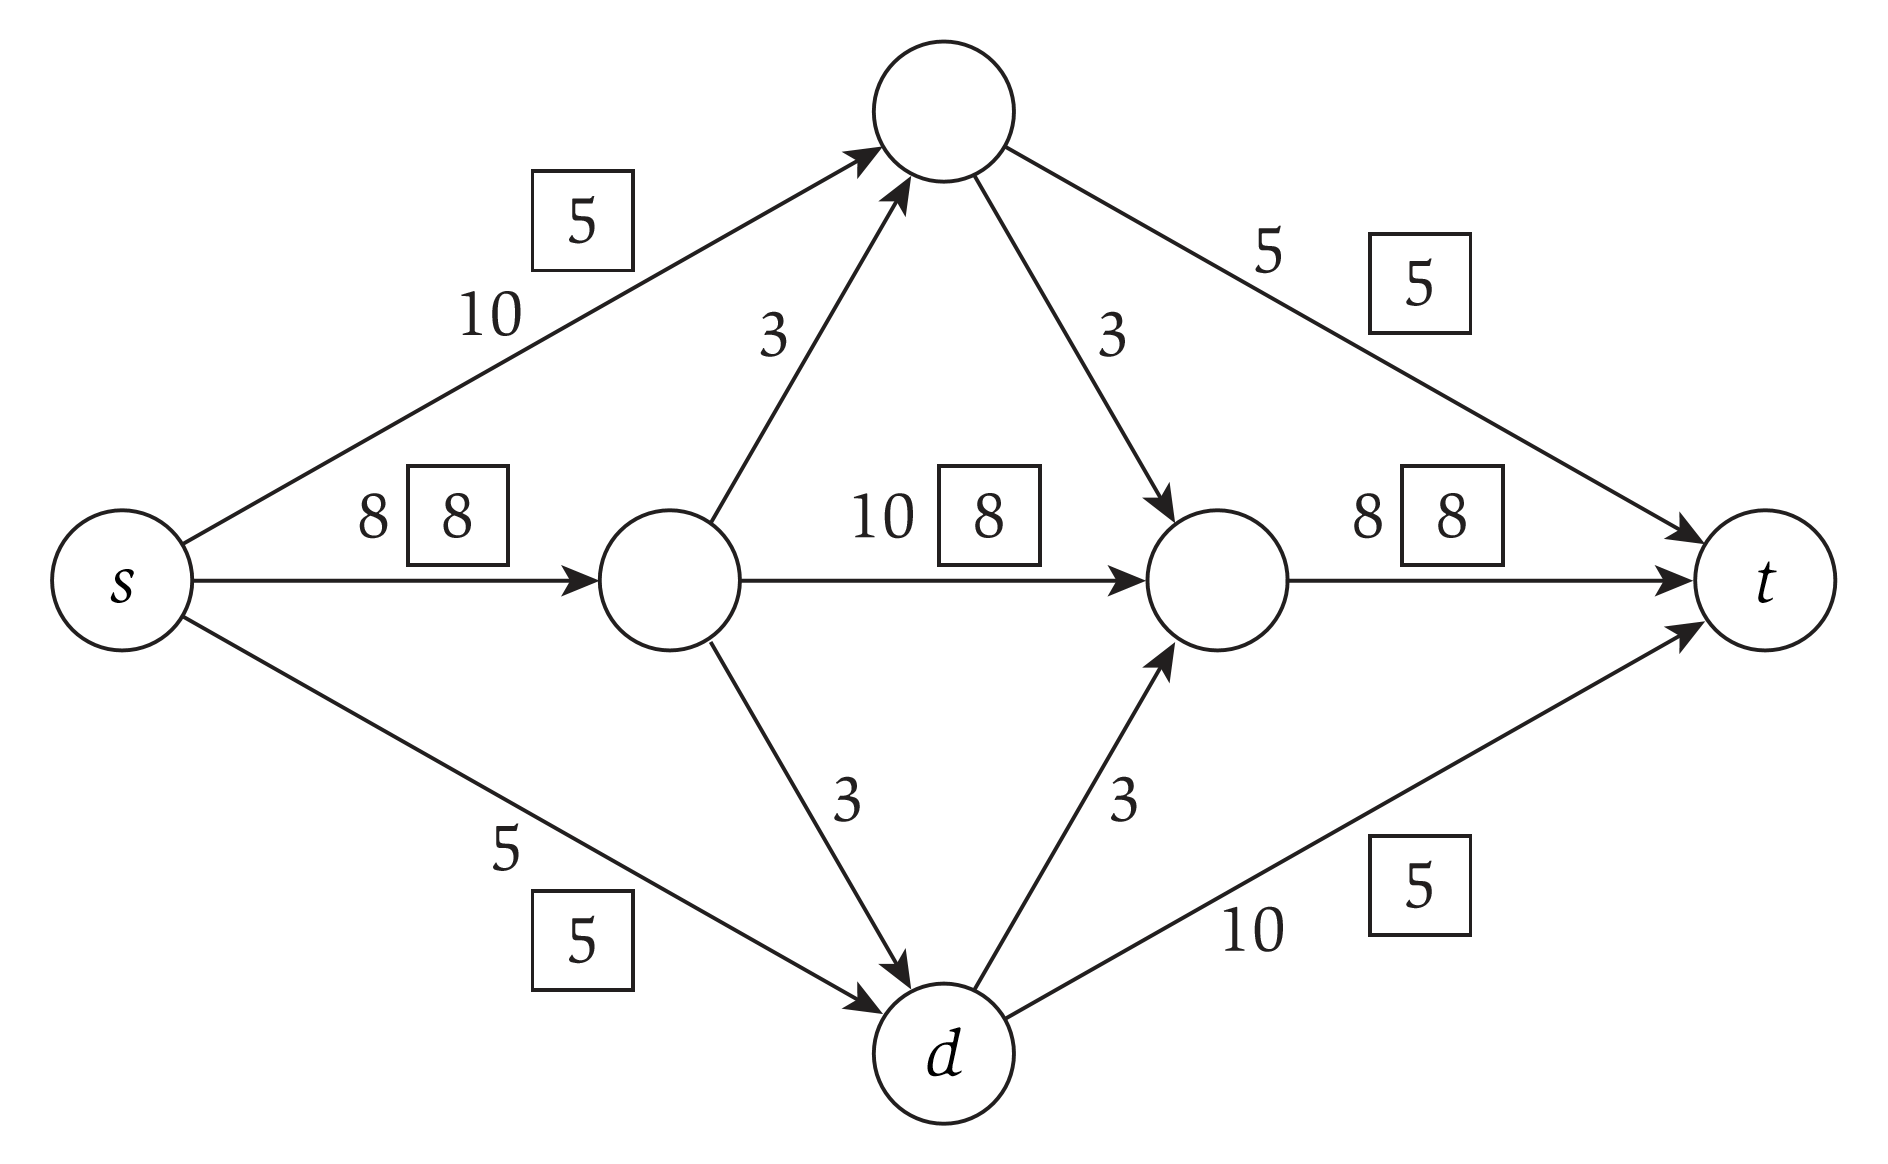
\includegraphics[width=0.5\linewidth]{fig3.png}
    \caption{A flow network.}
    \label{fig3}
\end{figure}


~\\
\textbf{Solution.}\\
\begin{itemize}
\item [a)] $flow=\sum_{e\ out\ of\ s} f_e = 5+8+5=18$. \\ Not a maximum flow. \\ $maxflow=8+8+5=21$.
\item [b)] Figure \ref{fig4} shows the minimum cut. Its capacity is $5+3+8+5=21$. \begin{figure}[htb]\centering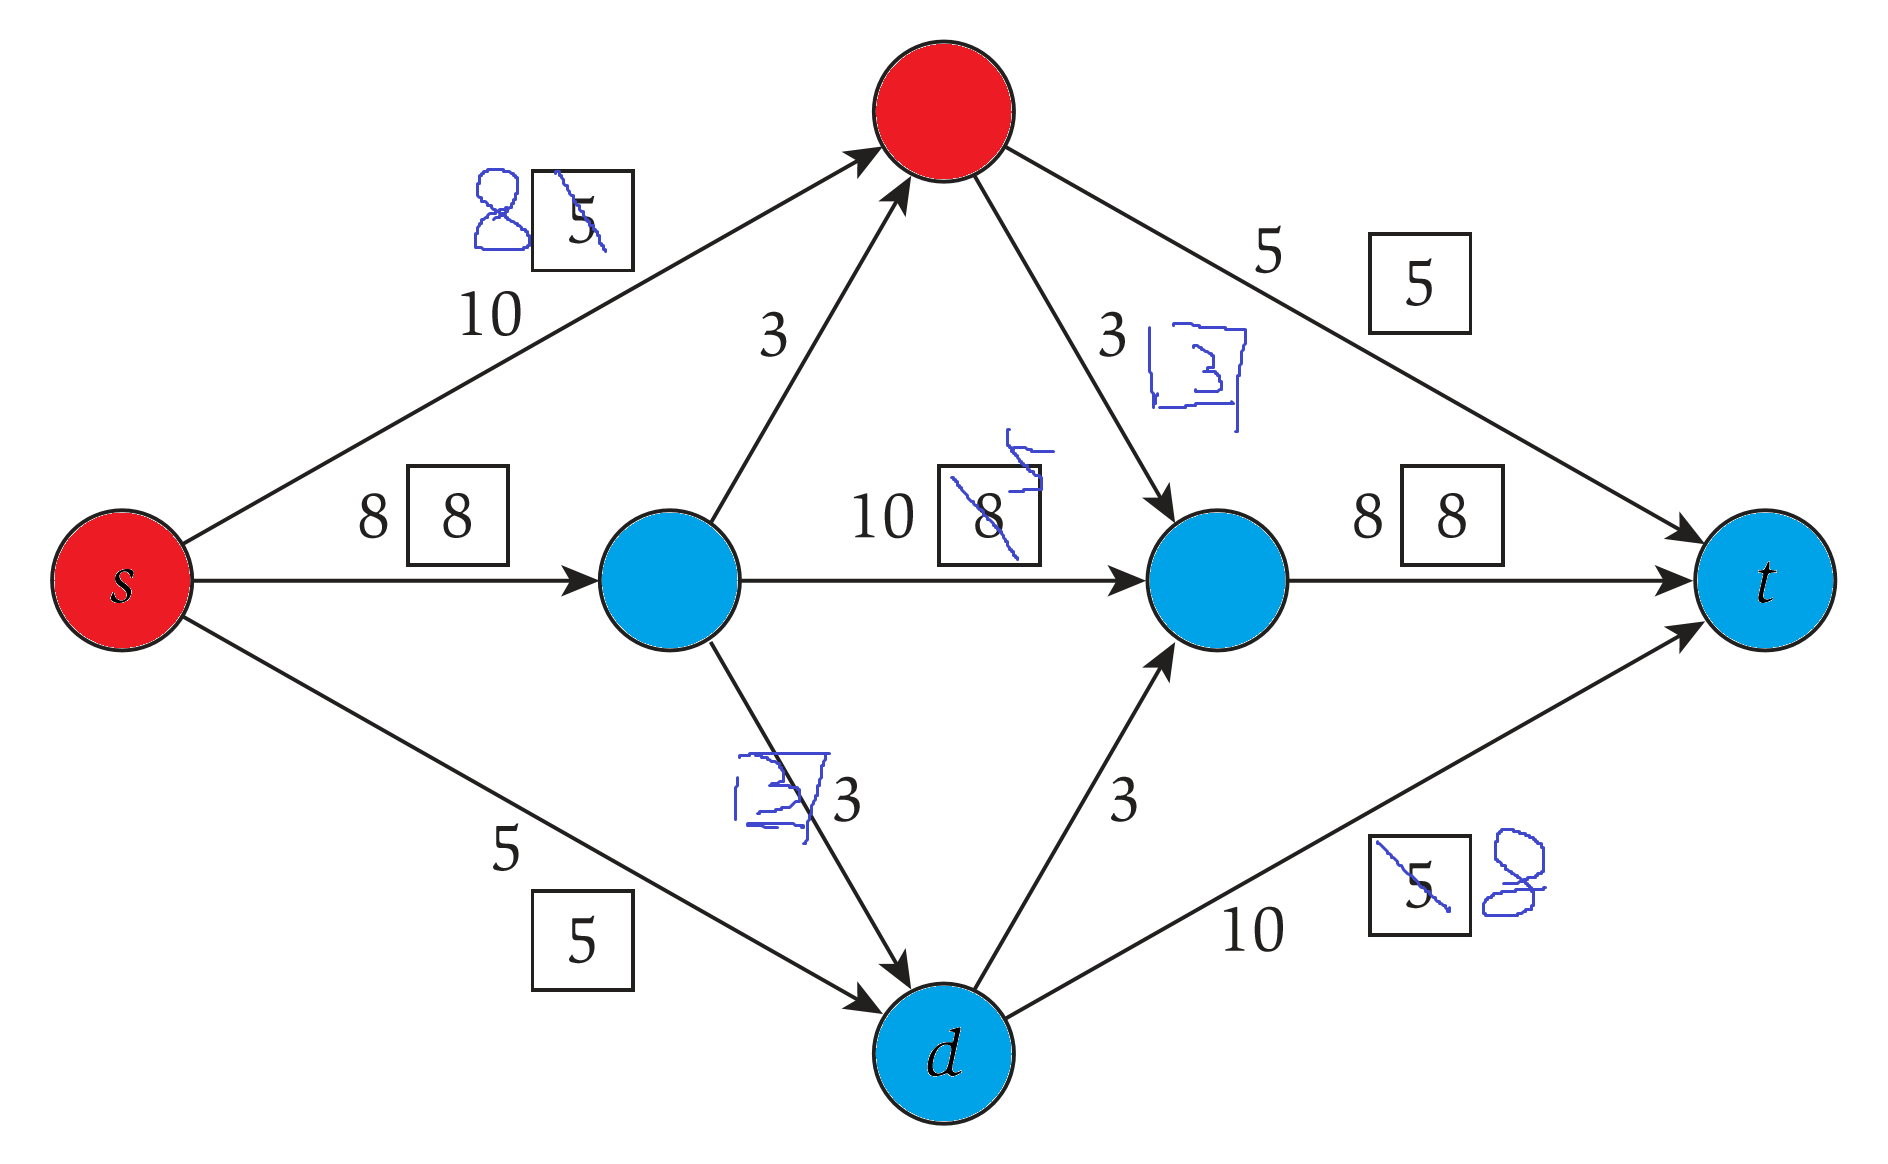
\includegraphics[width=0.5\linewidth]{fig4.png}\caption{minimum cut}\label{fig4}\end{figure}
\end{itemize}
~\\

\item We define the \textit{Escape Problem} as follows. We are given a directed graph $G=(V,E)$ (picture a network of roads). A certain collection of nodes $X \subset V$ are designated as \textit{populated nodes}, and a certain other collections $S \subset V$ are designated as \textit{safe nodes}. $X$ and $S$ are disjoint. In case of an emergency, we want evacuation routes from the populated nodes to the safe nodes. A set of evacuation routes is defined as a set of paths in $G$ so that (i) each node in $X$ is the head of one path, (ii) the last node on each path lies in S, and (iii) the paths do not share any edges. Such a set of paths gives a way for the occupants of the populated nodes to "escape" to safe nodes, without overly congesting any edge in $G$.

\begin{enumerate}
    \item Given $G$, $X$ and $S$, show how to decide in polynomial time whether such a set of evacuation routes exists.
    \item Suppose we have exactly the same problem as in (a), but we want to enforce an even stronger version of the "no congestion" condition (iii). Thus we change (iii) to say "the paths do not share any nodes". 
    
    With this new condition, show how to decide in polynomial time whether such a set of evacuation routes exists. 
    
    Also, provide an example with the same $G$, $X$ and $S$, in which the answer is yes to the question in (a) but no to the question in (b).
\end{enumerate}
~\\
\textbf{Solution.}\\
\begin{enumerate}
\item [(a)] We define such a network: \begin{enumerate}
    \item For $e\in E$, set the capacity of $e$ to $1$;
    \item Add a source $s$ and sink $t$;
    \item For each $v\in X$, add an edge $(s, v)$ with capacity $1$;
    \item For each $v\in S$, add an edge $(v, t)$ with capacity $+\infty$.
\end{enumerate}
Calculate the max flow on the network above, and check whether the max flow is equal to $|X|$. This can be finished within $O(|V|^2|E|)$ time. 
\item [(b)] We define such a network: \begin{enumerate}
    \item Add a source $s$ and sink $t$;
    \item Split each $v\in V$ into two nodes $v_i$ and $v_o$. And add an edge $(v_i, v_o)$ with capacity $1$;
    \item For each $(u,v)\in E$, add an edge $(u_o, v_i)$ with capacity $1$;
    \item For each $v\in X$ add an edge $(s, v_i)$ with capacity $1$;
    \item For each $v\in S$, add an edge $(v_o, t)$ with capacity $1$;
\end{enumerate}
Calculate the max flow on the network above, and check whether the max flow is equal to $|X|$. This can be finished within $O(|V|^2|E|)$ time. (In fact, splitting only the nodes in $V-X-S$ is OK).\\ Figure \ref{fig5} shows an example. 
\begin{figure}[htb]\centering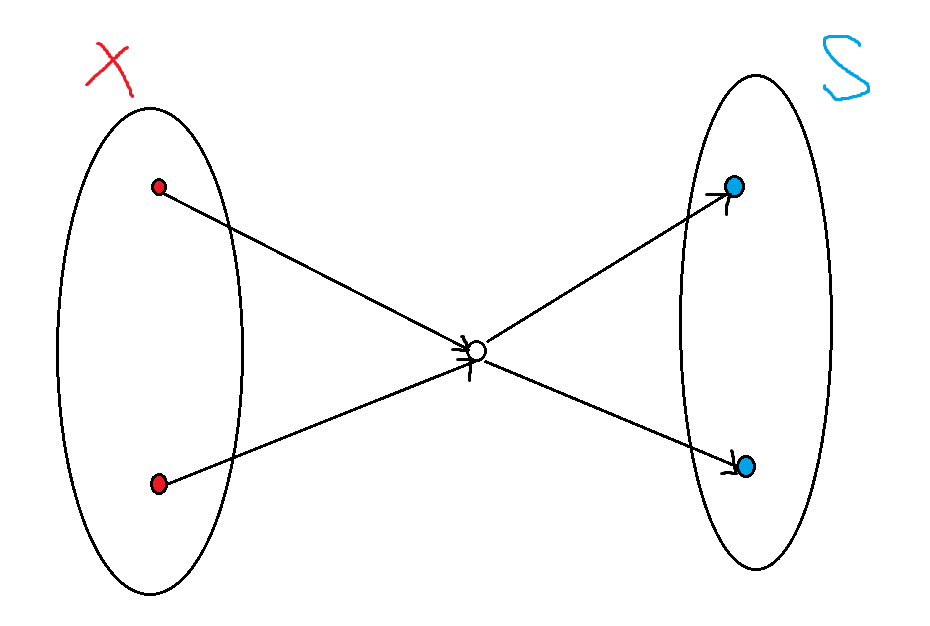
\includegraphics[width=0.5\linewidth]{fig5.png}\caption{example for 2.(b)}\label{fig5}\end{figure}
\end{enumerate}
~\\

\item Suppose there are n people living in a cooperative apartment. Over the next $n$ nights, each of you is supposed to cook dinner for the co-op exactly once, so that someone cooks on each of the nights.

Of course, everyone has scheduling conflicts with some of the nights, so deciding who should cook on which night becomes a tricky task. For concreteness, let's label the people $\{p_1, ..., p_n\}$ and the nights $\{d_1, ..., d_n\}$. For person $p_i$, there's a set of nights $S_i \subset \{d_1, ..., d_n\}$ when they are able to cook.

A feasible dinner schedule is an assignment of each person in the co-op to a different night, so that each person cooks on exactly one night, and there is someone cooking on each night. If $p_i$ cooks on night $d_j$, then $d_j \in S_i$.

\begin{enumerate}
    \item Describe a bipartite graph $G$ so that $G$ has a perfect matching if and only if there is a feasible dinner schedule for the co-op.
    \item There is a schedule constructed by your friend. Unfortunately, when you look at the schedule she created, you notice a big problem. $n-2$ of the people at the co-op are assigned to different nights on which they are available: no problem there. But for the other two people, $p_i$ and $p_j$, and the other two days, $d_k$ and $d_l$, you discover that she has accidentally assigned both $p_i$ and $p_j$ to cook on night $d_k$, and assigned no one to cook on night $d_l$. 
    
    You want to fix this mistake without having to recompute everything from scratch. Show that it's possible, using the "almost correct" schedule, to decide in only $O(n^2)$ time whether there exists a feasible dinner schedule for the co-op.
\end{enumerate}   


~\\
\textbf{Solution.}\\
\begin{enumerate}
\item [(a)] Define $V_1=\{p_1,p_2,\cdots,p_n\}, V_2=\{d_1,d_2,\cdots,d_n\}$, $E=\{(p_i,d_j)|d_j\in S_i\}$, and then $G=(V_1\cup V_2, E)$ is a reasonable bipartite.
\item [(b)] Just to check whether there is a augment path. We ignore the arrangement $(p_j, d_k)$ and define $E_1=\{(p_i,d_j)|d_j\in S_i\wedge (p_i,d_j)\ is\ not\ on\ schedule\}$, $E_2=\{(d_j, p_i)|(p_i, d_j)\ is\ on\ schedule\}$. Then we define a directed graph $G'=(V_1\cup V_2, E_1\cup E_2)$. Use BFS or DFS to check if there is a path from $p_j$ to $d_l$. If the path exists, then an augment path exists and hence there exists a feasible dinner schedule, otherwise not exist.\\ From the view of max flow algorithm, the $E_1\cup E_2$ is exactly the set of edges which has capacity $1$ and flow $0$.
\end{enumerate}
~\\

\item Recall that in the standard network flow problem we required that the for each vertex $v$ (excluding the source s and sink t) the sum of the flow into that vertex is equal to the sum of flow out of that vertex. Suppose that we replace this conservation constraint with a taxation constraint. In particular, suppose each vertex represents a country and that each country $v \notin  \{s, t\}$ has an associated tax-rate $0 < t_v < 1$ meaning that country $v$ will keep
$t_v$ fraction of the goods flowing through node $v$. Given a flow network $G = (V, E)$ with maximum capacities $c(e)$ on each edge $e \in V$ and tax rates $t_v$ for each node $v \notin {s, t}$ our goal is to find the maximum amount of goods that can be transported from $s$ to $t$ under these taxation constraints. Write down your algorithm to solve this problem. You should explain why your algorithm is correct. 

\textbf{Solution.}\\
\textbf{A naive thought}\\
I found that the order in which to find the augmented path impacts on the flow when there is a tax-rate $t_v$. So I have a simple thought that we should find the most effective augmented path in each turn. Move the tax rate from the node to the edge. For example, if there is an edge $(u,v)$, then the edge has transfer rate $1-t_u$, and its residual edge has transfer rate $(1-t_u)^{-1}$. In each turn, we find an augmented path with the largest accumulated transfer rate. For example, there is 4 nodes $1,2,3,4$, and 4 edges $(1,2),(2,4),(1,3),(3,4)$, and node $1$ has tax rate $0.5$, and node $2$ has tax rate $0.1$, and node $3$ has tax rate $0.2$. Then $1\rightarrow2\rightarrow4$ has accumulated transfer rate $0.5\times0.9=0.45$, and $1\rightarrow3\rightarrow4$ has accumulated transfer rate $0.5\times0.8=0.4$. We can use Bellman-Ford algorithm to find such a path with largest accumulated transfer rate (just take $\log$). But both the correctness and efficiency can be guaranteed in this naive solution: \begin{enumerate}
    \item I cannot prove that 'there is no augmented path' $\Rightarrow$ 'it is the max flow'. Max-flow min-cut theorem does not hold here.
    \item We do not find the shortest path. And the flow is not an integer. So the analysis of time complexity which is showed in class does not hold here.
\end{enumerate}
\textbf{A brute force solution}\\
I cannot come up with a solution related to graph theory on my own. So I am going to solve it with a brute force method. This is clearly an LP problem: \\
$$\min_f \sum_{e\ in\ t} f_e\ ,\ s.t.\left\{\begin{array}{ll}0\leq f_i\leq c_i ,&\forall 1\leq i\leq |E|\\\sum_{e\ out\ v} f_e = (1-t_v) \sum_{e\ in\ v} f_e ,&\forall v\in V.\end{array}\right.$$
The constraint matrix is sparse (at most 2 non-zero components in any column vector). It is suitable to use the simplex method (or interior point method) to solve the LP problem.\\ The main idea of simplex method is to go along the edge of the convex region to the direction of gradient descent. The detailed process is relatively complex to expand here, and I implement a naive simplex algorithm in my c++ code.
\end{enumerate}
Remark: You need to upload your .pdf file.

\end{document}
